% We started doing 1-page reports, so some layout stuff will have to be
% changed.  When asked what it's supposed to look like, Weatherford said it's
% ``memo format'' with 2 graphs and a brief conclusion.

% I (Charles) assume that means there's an abstract, results (just graphs,
% probably), and a short description/analysis of the results; the sections will
% be changed accordingly.

\documentclass{article}
\usepackage{graphicx}
\usepackage{float}
\usepackage[acronym]{glossaries}

\loadglsentries{acronyms}
\makeglossaries

% I'm not sure yet how to change the '/maketitle' output, so just
% leaving it alone for now.
\author{}
\title{ELEC 302-81\\ Lab 6\\ Separately Excited DC Motor}
\date{\today}

\begin{document}

\maketitle

\begin{center}
  \begin{tabular}{lr}
    Date Performed: & March 4, 2013 \\
    Partners: & Rawley Dent \\
              & Charles Pittman \\
    Instructor: & Dr. Weatherford
  \end{tabular}
\end{center}

\pagebreak

%\setlength\parindent{0pt}

\section{Abstract}

%In this experiment, the \gls{pm} and \gls{dyno} modules were used to measure
%torque, speed, power, and efficiency of a DC motor. This experiment consisted
%of three parts. Part 1 involved only the \gls{pm} module, and the basic

\section{Results}

% Stripped the title/legend from these graphs for two reasons: first, to save
% space; second, the title was wrong for the last plot, and it was easier than
% making a new one.
\begin{figure}[H]
  \centering
  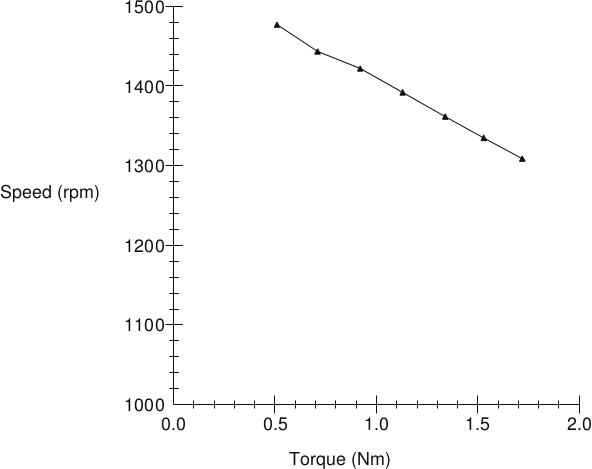
\includegraphics[width=\textwidth]{img/plot4}
  \caption{Speed vs. Torque}
  \label{fig:plot4}
\end{figure}

\begin{figure}[H]
  \centering
  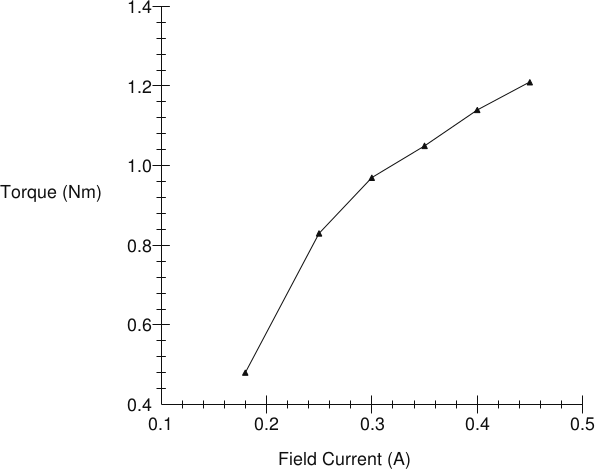
\includegraphics[width=\textwidth]{img/plot5}
  \caption{Torque vs. Field Current}
  \label{fig:plot5}
\end{figure}

\section{Conclusions}

%In Figure~\ref{fig:plot_02}, as the \gls{pm} was first starting to increase
%there was a large increase in torque in the opposite direction of motion.
%However, as the \gls{pm} gained rotational speed, the opposition torque

\end{document}
